%%!TEX root = ./UserManual.tex
\chapter{Visualiser}
\label{chap:visualiser}


%%%%%%%%%%%%%%%%%%%%%%%%%%%%%%%%%%%%%%%%%%%%%%%%%%%%%%%%%%%%%%%%
% Overview
%%%%%%%%%%%%%%%%%%%%%%%%%%%%%%%%%%%%%%%%%%%%%%%%%%%%%%%%%%%%%%%%
\section{Overview}
\label{section:overview}

\paragraph{} The Stride software includes a visualisation tool with which the disease spreading can be shown on a geographical map. When the visualiser is opened, the user is presented with a geographical map, a sidebar to the left and a toolbar on top. An overview can be seen in figure \ref{fig:screenshot_overview}

The toolbar contains various controls:
\begin{itemize}
\item Open file: Opens a open file dialog.
\item Save file: Opens a save to image file dialog.
\item Select Radius: Opens the radius selection dialog.
\item Select Rectangle: Opens the rectangle selection dialog.
\item Play-button: Enables/disables the automatic playback of the simulation results.
\item Timestep-slider: Allows the user to select a certain timestep of the simulation.
\item Health status dropdown: Allows the user to select a health status that is to be displayed.
\end{itemize}

%%%% IMAGE: overview

\begin{figure}[H]
\centering
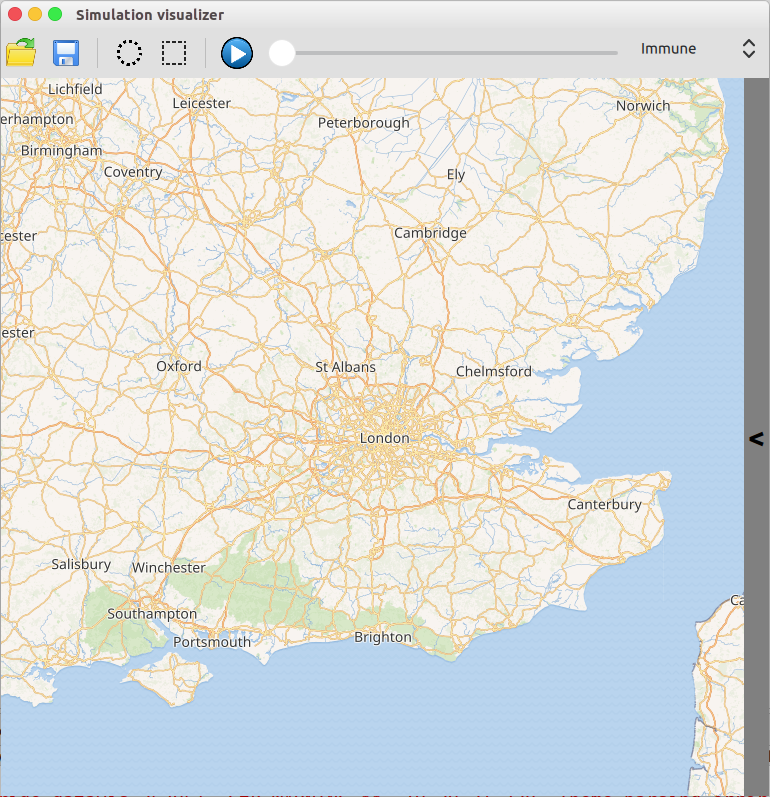
\includegraphics[width=0.7\textwidth,keepaspectratio]{images/overview.png}
\label{fig:screenshot_overview}
\caption{Overview of the visualisation tool}
\end{figure}

%%%%%%%%%%%%%%%%%%%%%%%%%%%%%%%%%%%%%%%%%%%%%%%%%%%%%%%%%%%%%%%%
% Epioutput
%%%%%%%%%%%%%%%%%%%%%%%%%%%%%%%%%%%%%%%%%%%%%%%%%%%%%%%%%%%%%%%%
\section{Epioutput}
\label{section:epioutput}
The visualiser is capable of loading files with epidemiological data, generated using stride. These files are referred to as 'epioutput' files, and can be used in three formats. They are generated by stride if provided with an appropriate configuration file. In order to generate an epioutput file, there are three parameters that can be set in the configuration file:

\begin{compactdesc}
\item [output\_epi] \ \\
    This parameter takes a boolean value indicating whether or not epioutput should be generated. Defaults to \emph{false}.
\item [output\_epi\_format] \ \\
    This parameter indicates the desired format for the epioutput. Currently supports '\emph{json}' and '\emph{hdf5}'.
\item [output\_epi\_interval] \ \\
    This parameter can be used to set an interval between recorded timesteps, e.g. and interval of 10 will capture the data once every 10 timesteps in the stride simulation. Defaults to 1.
\end{compactdesc}

The exact layout of the data depends on the format used, though all formats are similar. Generally, the file will contain a collection of timesteps. Each timestep will contain data about every location, more specifically, the health statuses of every \emph{ContactPoolType} in that location as well as its geographical data. This way, the visualiser can extract and display this data.


%%%%%%%%%%%%%%%%%%%%%%%%%%%%%%%%%%%%%%%%%%%%%%%%%%%%%%%%%%%%%%%%
% Viewing simulations
%%%%%%%%%%%%%%%%%%%%%%%%%%%%%%%%%%%%%%%%%%%%%%%%%%%%%%%%%%%%%%%
\section{Viewing simulations}
\label{section:viewing}

%%% IMAGE: open file
\begin{figure}[H]
\centering
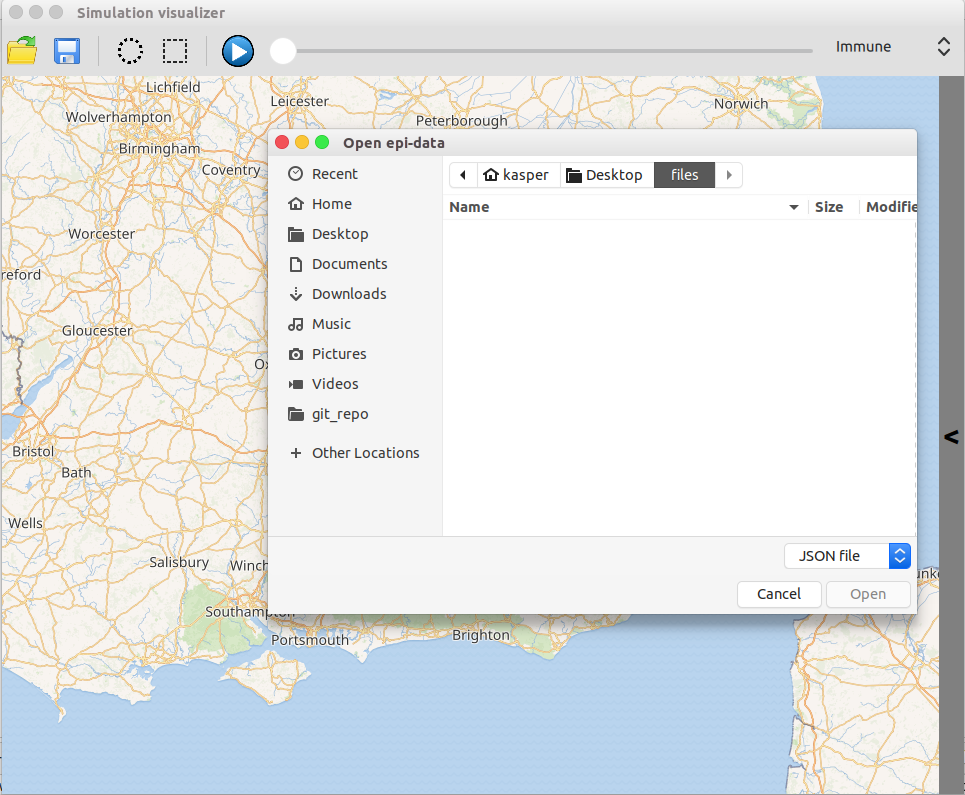
\includegraphics[width=0.7\textwidth,keepaspectratio]{images/open_file.png}
\label{fig:screenshot_openFile}
\caption{The open file dialog}
\end{figure}

%%% IMAGE: view simulation
\begin{figure}[H]
\centering
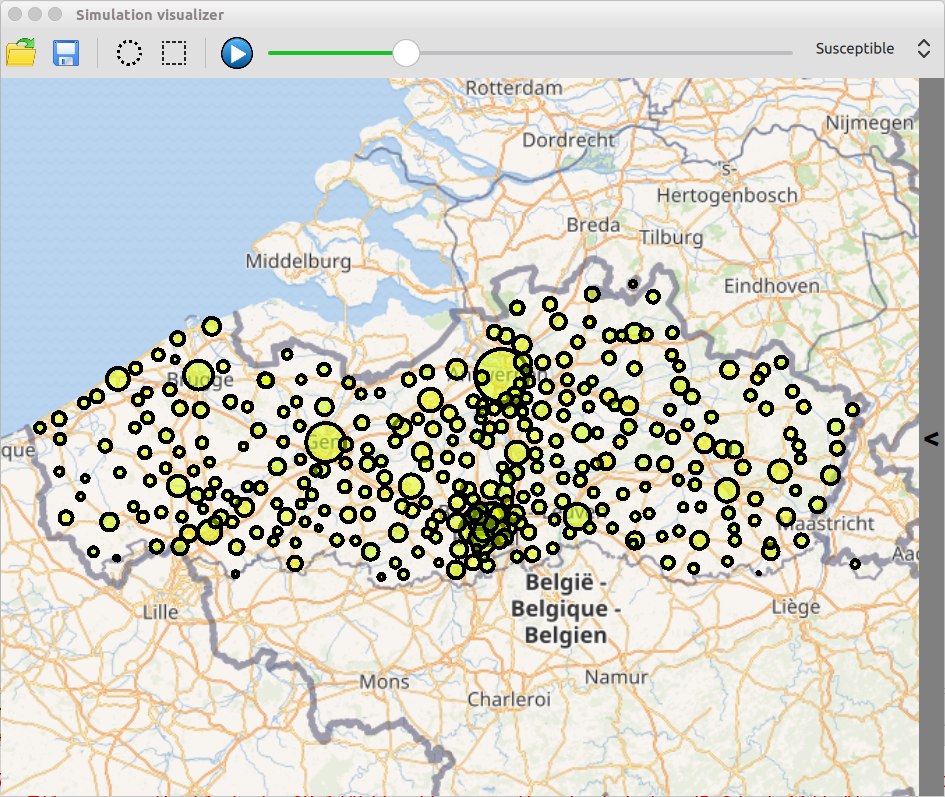
\includegraphics[width=0.7\textwidth,keepaspectratio]{images/view_simul.png}
\label{fig:screenshot_viewSimul}
\caption{The visualiser after a simulation has been opened}
\end{figure}



%%%%%%%%%%%%%%%%%%%%%%%%%%%%%%%%%%%%%%%%%%%%%%%%%%%%%%%%%%%%%%%%
% Selecting and viewing statistics
%%%%%%%%%%%%%%%%%%%%%%%%%%%%%%%%%%%%%%%%%%%%%%%%%%%%%%%%%%%%%%%
\section{Selecting and viewing statistics}
\label{section:stats_selection}

%%% IMAGE: view location stats
\begin{figure}[H]
\centering
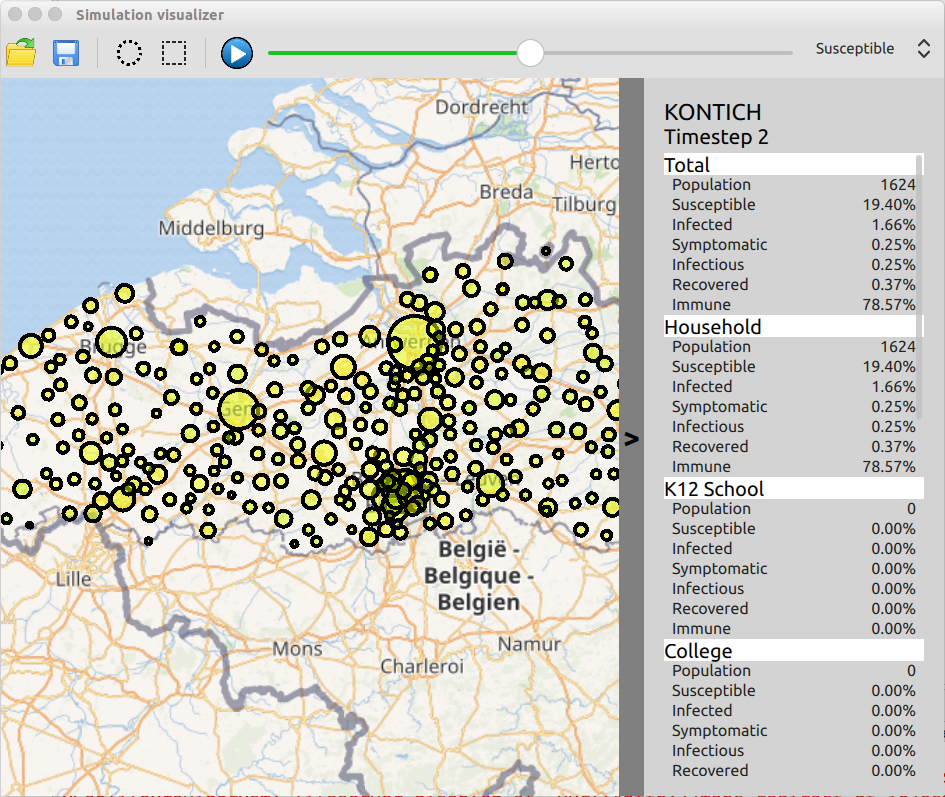
\includegraphics[width=0.7\textwidth,keepaspectratio]{images/stats_loc.png}
\label{fig:sceenshot_statsLoc}
\caption{The sidebar displaying statistics for the clicked location}
\end{figure}

%%% IMAGE rad selection
\begin{figure}[H]
\centering
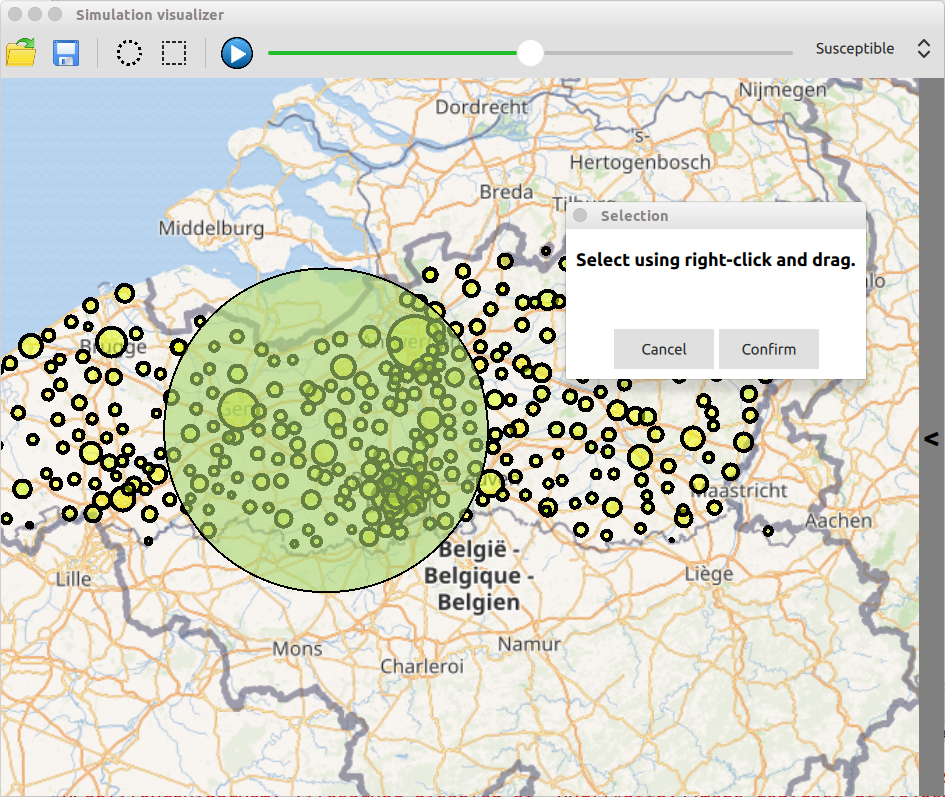
\includegraphics[width=0.7\textwidth,keepaspectratio]{images/select_rad.png}
\label{fig:screenshot_selectRad}
\caption{Radius selection}
\end{figure}

%%% IMAGE rect selection
\begin{figure}[H]
\centering
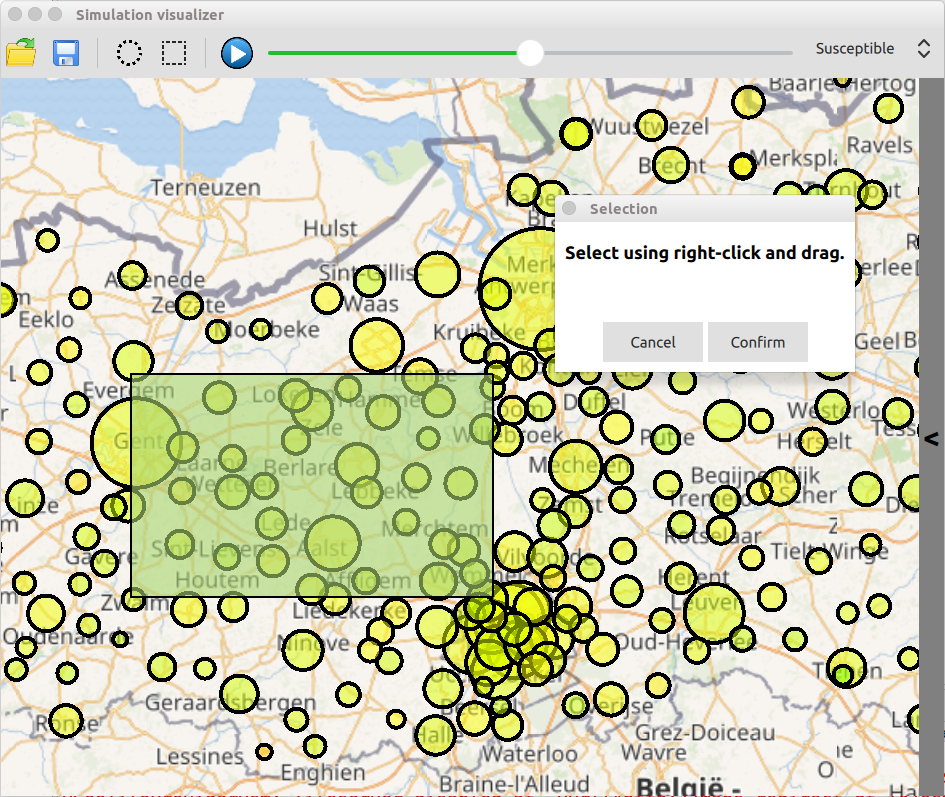
\includegraphics[width=0.7\textwidth,keepaspectratio]{images/select_rect.png}
\label{fig:screenshot_selectRect}
\caption{Rectangular selection}
\end{figure}


%%%%%%%%%%%%%%%%%%%%%%%%%%%%%%%%%%%%%%%%%%%%%%%%%%%%%%%%%%%%%%%%
% Exporting to image
%%%%%%%%%%%%%%%%%%%%%%%%%%%%%%%%%%%%%%%%%%%%%%%%%%%%%%%%%%%%%%%%

%%% IMAGE save to selection

\section{Exporting to image}
\label{section:export_image}


